\chapter{StackSync Reference Architecture}

Personal Cloud storage services have become commonplace but currently, 
commercial existing offerings are proprietary, and open source alternatives
are not mature enough. Researchers and practitioners interested in
pursuing Personal Cloud questions have few tools with which to work. 
Clearly, the lack of research tools is unfortunate given that most
fundamental questions are still unanswered: \textit{What is the appropriate
distributed architecture for a Personal Cloud? How do we manage versions
so that versioning is flexible, correct and scalable? What types of service level
agreements should a Personal Cloud service provide?} This is the basic 
reason why we have developed StackSync, an open source software framework
that implements the basic components of what is commonly referred to as a Personal Cloud.
All source code and data traces are available in \url{https://github.com/cloudspaces/stacksync}. 
Both the server and client code has been developed in Java:  The client is a branch from
the Syncany \cite{syncany} project and the server is using our novel communication middleware called
ObjectMQ~\cite{omq} that will be presented in brief. The implementation currently has approximately
$33,000$ lines of code, distributed in the following way: 1. \textit{ObjectMQ middleware} \textemdash~$2,100$ lines; 
2. \textit{StackSync client} \textemdash~$24,400$ lines; and
3. \texttt{SyncService} \textemdash~5,800 lines.

Indeed, an important design decision of our reference implementation was to rely on a messaging middleware for communication. 
Since Personal Cloud storage services exhibit significant read-write ratios~\cite{Dropbox}, we decided that the sync
engine should support \textit{persistent client connections, push-based notifications, and asynchronous and stateless interactions}.
A message-oriented middleware fits well with these requirements, because of its support to \textit{loosely coupled communication}
among distributed components thanks to \textit{asynchronous message-passing}.

StackSync is currently using RabbitMQ as its message broker and PostgreSQL as its default \texttt{Metadata back-end}. By default, 
we use OpenStack Swift as \texttt{Storage back-end}, though others are also possible. Indeed, the StackSync framework presents extension
hooks that enable others to replace the \texttt{Storage back-end}, the \texttt{Metadata back-end}, the message broker, 
the synchronization protocol or even the chunking and deduplication strategies.


An overview of our architecture with the main components is shown in Fig.~\ref{fig:architecture}. 
The StackSync client and the \texttt{SyncService} interact through the ObjectMQ middleware layer abstracting
the RabbitMQ message broker.  The \texttt{SyncService} interacts with the \texttt{Metadata back-end}. The StackSync client directly interacts with the \texttt{Storage back-end} to upload and download chunks. Finally, the REST API is used for accessing storage and sharing services from mobile
and web clients. Security components like the authentication and authorization services are not included here.

\begin{figure}[t]
\centering
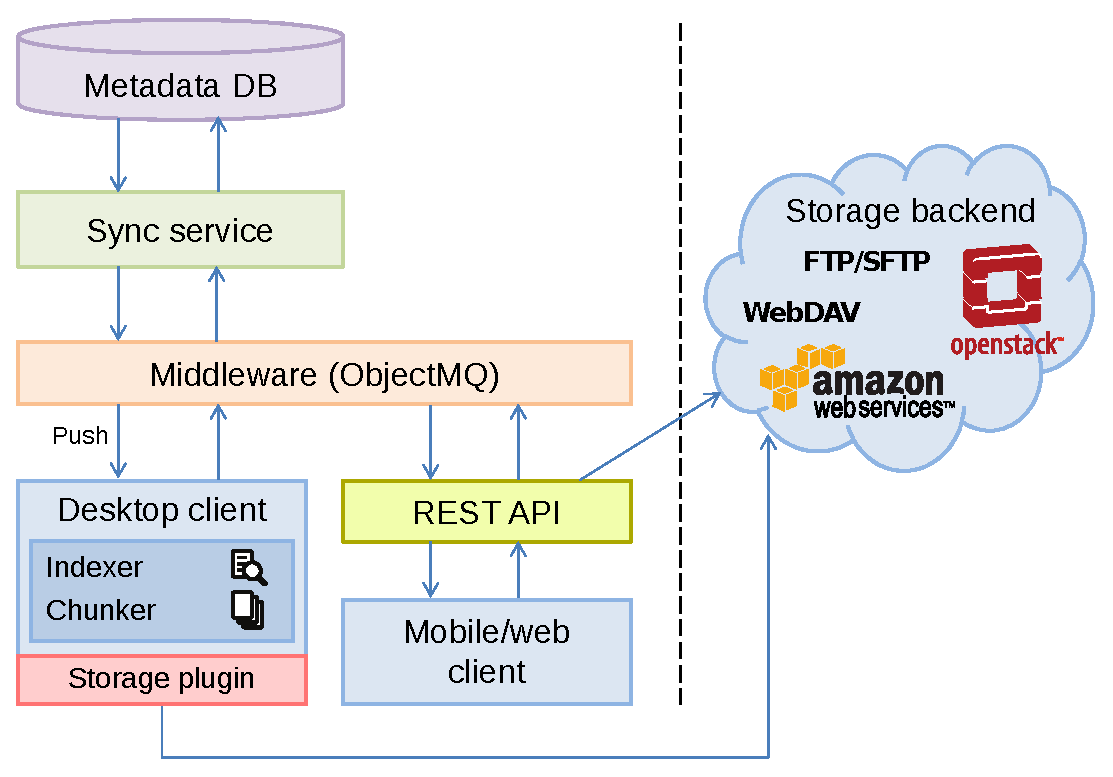
\includegraphics[width=0.75\textwidth]{figures/big_picture_v2}
\caption{StackSync architecture}\label{fig:architecture}
\end{figure}

\subsection{StackSync Synchronization Protocol}

Since file synchronization lies at the heart of any Personal Cloud service, 
we present a reference synchronization protocol that is available in the StackSync framework,
whose main novelty is that it is based on a \textit{message-oriented middleware} (MOM). In particular, 
MOM is ideally suited here for:

\begin{enumerate}
\item \textit{Scalable change notification:} The high read-write ratio of Personal Cloud services makes
it more appropriate to employ \textit{one-to-many push communication} for quickly notification.  
Server-based protocols like this are required when replicas need a high degree of consistency \cite{Tanenbaum:2001:DSP:559404}.
\item \textit{Asynchronous message dispatching:}  Synchronization operations require significant
server processing time for ensuring consistency. Decoupling message dispatching from message
processing in these scenarios  \cite{menasce2005mom} is important for scalability reasons.
\item \textit{Implicit load balancing:} When many consumers read from a queue, messages are
distributed among them. This way, we can start multipe
instances of the \texttt{SyncService} to alleviate the load of the incoming request queue,
\textit{allowing to scale up and down very easily as computing needs change}.
\end{enumerate}

Let us describe the overall synchronization protocol:
\medskip

\subsubsection{Communication middleware}
Our reference architecture relies on a high-performance message broker compatible with the Advanced Message Queueing Protocol (AMQP)~\cite{amqp} standard. In order to simplify the interaction with this messaging middleware, we have built the ObjectMQ communication middleware. 

ObjectMQ is a lightweight remote object layer constructed on top of a messaging middleware compatible with AMQP~\cite{amqp}. 
We are combining RPC and MOM models to devise four MOM-RPC invocation abstractions: \textit{two one-to-one calls} (synchronous, 
asynchronous) and \textit{two one-to-many calls} (multi, event).

In general, objects receive method calls as messages in incoming queues, and then reply the results to clients in response queues.  
One-to-many calls are distributed using the appropriate AMQP Exchanges (broker message dispatchers). Recall that Exchanges determine
message delivery and provide different delivery schemes, like \textit{direct} (deliver this message to a particular queue) and \textit{publish-subscribe}
(deliver this message to all queues subscribed to a certain topic). Let us define the four calls:

\begin{itemize}

\item @async:  This is an asynchronous non-blocking  one-way invocation where the client  publishes a message in the target object request 
Queue ($Q_{Request}$). By default, the client expects to receive no response and it is even not notified if the message was handled correctly.


\item @sync:  This is a synchronous blocking remote call where the client publishes a message in the target object
request Queue ($Q_{Request}$), blocking until a response is received in its own client response queue ($Q_{Response}$).  
This call can be configured with a timeout and a number of retries to trigger the exception if the result does not arrive.

\item @event:  This is an asynchronous non-blocking one-to-many notification triggered by a server.  The server triggers an @event by publishing the message in  the Event  fan-out Exchange ($E_{Event}$). Any client subscribing to this event in the server must bind their incoming Event Queue ($Q_{Event}$) to the server Exchange ($E_{Event}$).

\item @multi: This is an asynchronous non-blocking one-to-many invocation from one client to many servers. The clients invokes the method in all servers by publishing an event in the Multi  fan-out Exchange ($E_{Multi}$). All servers bind their incoming Request Queue ($Q_{Request}$) to the Multi Exchange ($E_{Multi}$).

   
\end{itemize}


The ObjectMQ communication middleware supports different compression and transport protocols (Kryo~\cite{kryo}, Java Serialization, JSON). It also handles transparently all the error management and communication services on top of the MOM broker. We outline that the initial code of the StackSync client has been reduced in around $3,000$ lines of code after introducing our ObjectMQ communication library. 

Finally, it is worth mentioning that our communication middleware could be easily replaced by a ``traditional'' RPC layer using a pull approach for change notification. Although our reference implementation is based on messaging and the push model, the StackSync framework is also open in the 
communication layer.


\subsubsection{SyncService and metadata back-end}

The \texttt{SyncService} is a server-side component implemented as a remote object using the ObjectMQ communication middleware. This service directly benefits from the invocation abstractions offered by ObjectMQ. 


\begin{figure}[t]
\centering
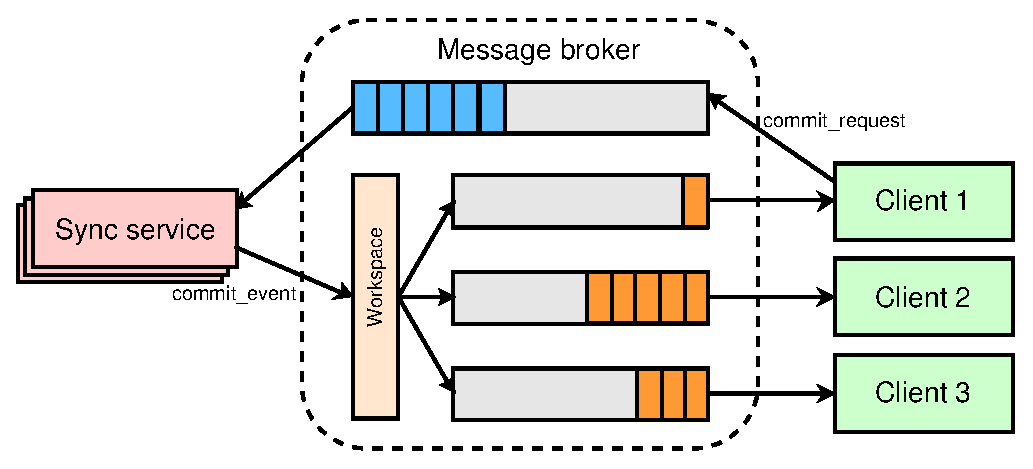
\includegraphics[width=0.66\textwidth]{figures/message_broker}
\caption{Message broker communication flow}\label{fig:message_broker}
\end{figure}


In our current design (see Fig.~\ref{fig:message_broker}), ObjectMQ is using a global request queue for the \texttt{SyncService}, 
a response queue for each device (\texttt{SyncService} Proxy), and a fan-out  Exchange for each workspace.  Each device will bind its request queue to the appropriate workspace Exchange to receive notification changes in this workspace.  In any case, queue message programming is abstracted thanks to ObjectMQ, so that the protocol will be defined in terms of RPCs or method calls.
\vspace{-10pt}

\begin{figure}[h!]
\lstset{language=Java, showstringspaces=false, tabsize=3, basicstyle=\scriptsize,frame=single, captionpos=b, basewidth=0.44em, commentstyle=\color{green}}
\begin{lstlisting}
	@RemoteInterface
	public interface SyncService extends Remote {

    	@SyncMethod(retry = 5, timeout = 1500)
    	public List<ObjectMetadata> getChanges(Workspace workspace);

    	@SyncMethod(retry = 5, timeout = 1500)
    	public List<Workspace> getWorkspaces();

    	@AsyncMethod
    	public void commitRequest(Workspace workspace, List<ObjectMetadata> objectsChanged);

	}
	@event
	public interface CommitEvent extends Event {
		
		public List<ObjectMetadata> objectsChanged getChanges();
	}
	
		\end{lstlisting}
		\caption{SyncService interface}
		\label{fig:idl}
\label{Code:push}
\vspace{-10pt}
\end{figure}

In Fig.~\ref{fig:idl} we can see the interface definition of the \texttt{SyncService}. Clients can request the list of Workspaces they have access to with the \textit{getWorkspaces} operation. Once the client obtains the list of Workspaces, it can then perform two main operations: \textit{getChanges} and  \textit{commitRequest}. Furthermore, the client will be notified of changes  by means of the event \textit{CommitEvent}.

\texttt{getChanges} is a synchronous operation (@sync) that StackSync clients perform on startup. This is a costly operation for the \texttt{SyncService} as it returns the current state of a Workspace. Once the client receives this information, it registers its interest in receiving committed updates, i.e., \textit{CommitEvent}s (@event) for this Workspace. From that point on, any change occurring on this Workspace will be notified to the client in a push style.

\texttt{commitRequest} is an asynchronous operation (@async) that clients employ to inform the \texttt{SyncService} about
detected file changes in their Workspaces.  This is a  costly operation since it must guarantee the consistency of data after the new changes. 

\texttt{CommitEvent} is triggered by the \texttt{SyncService} in  an asynchronous one-to-many operation (@event) to all out-of-sync devices in the specified Workspace. This operation is only launched by the \texttt{SyncService} once the changes has been correctly stored in the \texttt{Metadata back-end}.

\begin{algorithm}[h]
  \caption{Pseudocode of the commitRequest function in the SyncService}
    \label{alg:commit_pseudocode}
  \begin{algorithmic}[1]
  	\footnotesize
    \Function{commitRequest}{$workspace, List<ObjectMetadata> objects\_changed$}
      \State $commit\_event \gets $ new instance of CommitEvent
      \For{$new\_object$ \textbf{in} $objects\_changed$}
      	\State $server\_object \gets metadata\_backend.get\_current\_version(new\_object.id)$
        \If {\textbf{not exists} $server\_object$}
          	\Comment To commit the first version of the new object
        	\State $metadata\_backend.store\_new\_object(new\_object)$
        	\State $commit\_event.add(new\_object, \mathtt{confirmed} = True)$
        \ElsIf{$server\_object.version$ \textbf{precedes} $new\_object.version$}
         	\\ \Comment No conflict, committing the new version
			\State $metadata\_backend.store\_new\_version(new\_object)$
			\State $commit\_event.add(new\_object, \mathtt{confirmed} =True)$
        \Else
        	\\
        	\Comment Conflict detected, the current object metadata is returned
        	\State $commit\_event.add(new\_object, \mathtt{confirmed} = False,  server\_object)$
        \EndIf
      \EndFor 
      \State $trigger\_event(workspace, commit\_event)$
    \EndFunction
  \end{algorithmic}
\end{algorithm}

Algorithm~\ref{alg:commit_pseudocode} reports the pseudocode of the \texttt{commitRequest} operation. When a \texttt{commitRequest} message is received in the global request queue, the ObjectMQ middleware will invoke the appropriate \texttt{commitRequest} method in the \texttt{SyncService}. 
This method then receives a proposed list of change operations in a concrete Workspace. For every change operation, it will then check if the current version of the object in the \texttt{Metadata back-end} precedes the change proposed by the client. In this case, the changes are (transactionally) stored in the \texttt{Metadata-back-end} and confirmed in the \texttt{CommitEvent}. If there is a conflict with versions, the \texttt{commitRequest} is set as failed and information about the current object version is added to the \texttt{CommitEvent}. The reason for adding the current object version to the \texttt{CommitEvent} is
to piggyback the information about the ``differences'' between the two versions, such that the ``losing'' client can identify the missing chunks and
reconstruct the object to the current version. 
As usual, in StackSync, a conflict occurs when two users change a file at the same time. This implies that the two clients
will propose a list of changes over the same version of the file. The first \texttt{commitRequest} to be processed will
increase the version number by one, but the second \texttt{commitRequest} will inevitably propose a list of changes over
a preceding version, resulting in a conflict. 

To resolve the conflict, the \texttt{SyncService} adopts the simplest policy in this case, which is to consider as 
the ``winner''  the client whose \texttt{commitRequest} was processed first. This way, the \texttt{SyncService}
avoids rolling back any update to the \texttt{Metadata back-end}, saving time and increasing scalability. At the client,
the conflict is resolved by renaming the ``losing'' version of the file to ``... (conflicted copy, ..)''.

Finally, the \texttt{CommitEvent} will be triggered to the Workspace AMQP Exchange, and 
it will be received by all interested devices in their incoming event queues. 

As just elaborated above, note that the \texttt{CommitRequest} is an important operation in the sync service since it has to provide \textit{scalable request processing, consistency, and scalable change notification}.  Scalable request processing is achieved because the method is \textit{asynchronous} and \textit{stateless}. Multiple \texttt{SyncService} instances can listen from the global request queue and the message broker will transparently
balance their load. Consistency is achieved using the transactional  ACID model of the underlying \texttt{Metadata back-end}. 
Finally, scalable change notification to the interested parties is achieved using one-to-many push notifications (@event).

The \texttt{SyncService} interacts with the \texttt{Metadata back-end} using an extensible Data Access Object. Our reference implementation is based on a relational database although the system is modular and may be replaced easily.



\subsubsection{StackSync Client and Storage back-ends}


The StackSync client is a local Java library that monitors the local folder and synchronizes it with a remote repository. 
As described before, the StackSync client now interacts with two main remote services: the \texttt{SyncService} 
through the ObjectMQ middleware, and with different \texttt{Storage back-end}s to upload and download chunks.

This decoupling of sync control flows from data flows implies that the client must authenticate with both entities. But it also enables a user-centric design where the client directly controls its digital locker or storage container.  The synchronization protocol have been designed to put the load in the client side, whereas the \texttt{SyncService} just checks if the change is consistent, and then apply all changes proposed by clients. 

Every client has a local database and a \texttt{Watcher} thread that monitors the state of the sync folders.  On startup, the client must ask the server for its list of workspaces and its current state. From that point on, the \texttt{Indexer} will be notified by the \texttt{Watcher} of  changes in the local folder and it will periodically send them using the \textit{commitRequest} operation. Besides that, the client can receive commit events (\textit{commitChanges}) from the server that will be immediately applied to the local workspace.  Regarding potential conflicts due to offline operations, we provide similar policies than Dropbox, so that we create a copy of the conflicted document and let the user decide about this. 


To save storage space and bandwidth, the \texttt{Indexer} uses source-based deduplication at the block
level to store and transmit only a single copy of each duplicate block to the server. In our
reference implementation, deduplication is applied on a per-user basis, as cross-user
deduplication has been proven to be insecure~\cite{harnik10}. This means that deduplication is carried out
separately for each user, and therefore, data blocks of other users are not utilized to detect
if an identical copy of the block is already at the server. Specifically, the client software
maintains a chunk database to identify and locate duplicate data chunks. The database indexes
each chunk by its fingerprint, which by default is the 20 bytes of its SHA-1 hash, though weaker
fingerprints like the 32-bit Adler32 checksum may be used to reduce the index size. The database
maintains the information of the chunks that form each file, so that whenever a file is
modified, the client avoids transferring duplicate blocks to the server. Thanks to our message-
oriented sync protocol, keeping such a database in sync with the server is inexpensive, as any
changes on the central storage are advertised by means of asynchronous \textit{CommitEvent}s as soon as
they are performed.

StackSync's \texttt{Chunker} currently supports both fixed-sized and content-based chunking. Fixed-size chunking partitions a
file into fixed-size blocks. Although fixed-size chunking does not perform well due to the
boundary-shifting problem~\cite{Eshghi05}, it is useful to keep it as it incurs significantly lower
computational costs that their content-based counterparts. For content-based chunking, StackSync
supports Rabin-based chunking~\cite{Muthitacharoen01} and the Two-Threshold Two-Divisor (TTTD) chunking
algorithm~\cite{Eshghi05}. TTTD produces variable-sized chunks with smaller size variation than other
chunking algorithms, leading to superior deduplication. In any case, the chunks are compressed
before transmission using Gzip or Bzip2, albeit other compression algorithms can be easily
plugged into the architecture.

Finally, and based on the original Syncany architecture, we provide an extensible plugin-based architecture for connecting to third-party \texttt{Storage back-ends}. We now provide plugins for Amazon S3, OpenStack Swift, Dropbox, WebDAV, SMB and FTP.  It is straightforward to provide new plugins and we aim to leverage the open source community of Syncany for adding additional plugins to our platform.